
 \documentclass[12pt,a4paper]{report}
 
 \usepackage[pagebackref=false,colorlinks,linkcolor=blue,citecolor=magenta]{hyperref}
 
 \usepackage[nottoc]{tocbibind}
 \usepackage{calc}
 \usepackage{eso-pic}
 \usepackage{hyperref}
 \usepackage {fancybox}
 \usepackage{graphicx, xcolor}
 
 \usepackage{xepersian}
 \settextfont{B Nazanin}
 \title{دیپ‌فیک ما را به کجا خواهد برد؟
 	
 	 خوب،بد و زشت دیپ‌فیک‌ها}
\author{ آقایان محمدرضا محمدی و رضا رضایی}
\renewcommand{\bibname}{مراجع}
\begin{document}

	\thisfancypage{\setlength{\fboxsep}{10pt}\doublebox}{}
	

 	\maketitle
 	\tableofcontents
	
	
	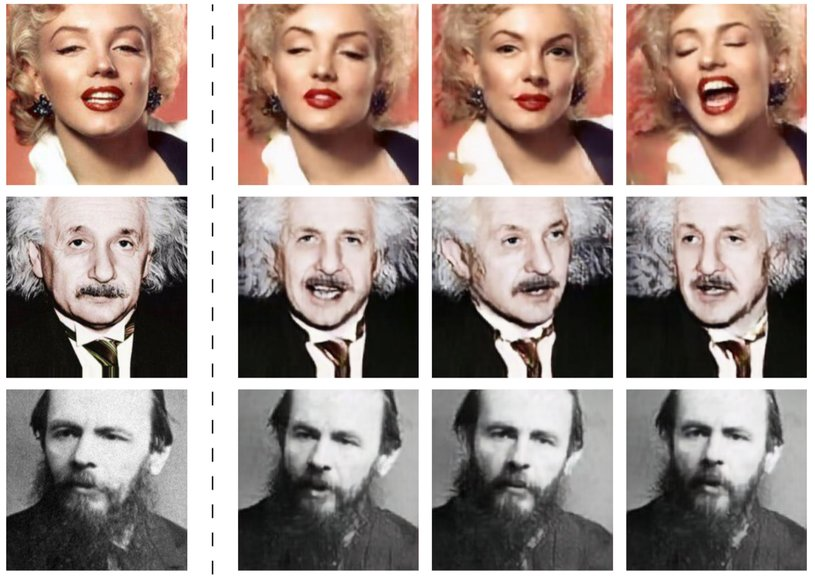
\includegraphics[width=1 \textwidth]{images/firstPic.jpeg}
	
 	
 	
 	\vspace{20pt}
 	
 	{\LARGE  مقدمه }
 	
 	{\large در یکی از صحنه‌های فیلم«اگه میتونی منو بگیر» \LTRfootnote{catch me,if you can} ساخته استیون اسپیلبرگ، یک مامور  \lr{FBI}\LTRfootnote{Federal Bureau of Investigation}  به نام کارل هنرتی در جستجوی کلاهبرداری به نام فرنک ابگنیل جونیور وارد اتاق او در هتل می‌شود. ابگنیل در همان حالتی که لوله تفنگ به سمت صورتش گرفته شده، وانمود می‌کند که مامور مخفی پلیس است و خودش هم دارد دنبال ابگنیل کلاهبردار می‌گردد. سرانجام ابگنیل موفق می‌شود سر هنرتی را شیره بمالد و درست جلوی چشمان حیرت زده او از چنگش دربرود. این فیلم که شخصیت اصلی‌اش مدام بین واقعیت و دروغ در تلاطم است، قصه بچه نابغه‌ای است که مسیر بدی را در پیش گرفته است. این روزها همین قصه را داریم در رسانه‌ها از نو زندگی می‌کنیم: همه‌ما هنرتی‌هایی هستیم که توانایی‌مان برای تشخیص راست از دروغ، حقیقت از کلک، و درست‌کاری از بدبینی به بازی گرفته شده است. کلاهبردار این قصه اگر گفتید کیست؟ بله، دیپ‌فیک‌ها\LTRfootnote{DeepFake}.
 	}
 	
\chapter{دیپ‌فیک چیست؟}\label{فصل اول }
\section{دیپ‌فیک از کجا می آید؟}
 	 کلمه دیپ فیک \lr{\textbf{Deepfake} } ترکیبی از \lr{deep learning } و  \lr{fake} به معنای یادگیری عمیق جعل کردن، تکنیکی برای تلفیق تصویر انسان بر اساس هوش مصنوعی است. این فناوری جهت ترکیب و قرار دادن تصاویر و فیلم های موجود بر روی تصاویر یا فیلم های مورد نظر با استفاده از تکنیک یادگیری ماشین تحت عنوان “شبکه مولد تخاصمی ” (\lr{\textbf{GAN}} )\LTRfootnote{Generative adversarial network}  بکار می رود. 
 		
 		
 		تلفیق تصاویر و فیلم های موجود با منبع مورد نظر ویدئویی به نحوی صورت میگیرد که گویی ترکیب هر دو تصویر یا هر دو فیلم یکی است و در یک صحنه رخ می دهد . این ترکیب پیچیده به طور مثال می تواند یک فرد یا افراد را به گفتن چیزها و یا انجام اقداماتی نشان دهد که هرگز در واقعیت رخ نداده اند.\cite{asrIran}
 		
 		
\section{\lr{GAN}}
 	 
 		گَن یک بخش \textcolor{blue}{«مولد» } دارد و یک بخش \textcolor{blue}{«ممیز»}. مثلا فرض کنید گَن قصه ما، یاد گرفته باشد تصویرهای دروغین از خلبان‌ها بسازد. مولد یا همان ابگنیل قصه، دارد سعی می‌کند عکس‌های تقلبی جعل کند. از آن طرف ممیز یا هنرتی داستان، عکس‌های جعلی ساخت مولد و عکس‌های واقعی را کنار هم می‌گذارد و به خودش یاد می‌دهد که عکس واقعی را از دروغی تشخیص دهد. هرچقدر که مدل گَن بیشتر یاد بگیرد، هر دو بخش‌های مولد و ممیز هم در کارشان بهتر عمل می‌کنند و هرکدام باعث می‌شود دیگری در کار خودش ماهرتر شود. دیپ‌فیک‌ها جعل‌هایی هستند که مولد بلاخره توانسته از زیر دماغ ممیز رد کند! \cite{queraMag} 
 		
شاید قبلا سایت \textcolor{blue}{«\href{https://thispersondoesnotexist.com/}{این فرد وجود خارجی ندارد}»} را دیده باشید؛ این سایت با کمک هوش مصنوعی، عکس پروفایل‌های آدم‌‌هایی را می‌سازد که هرگز وجود نداشته‌اند. چطوری؟ با الگوریتم شبکه مولد تخاصمی \lr{ (Generative Adversarial Network)} یا به طور خلاصه، گَن (\lr{GAN}). این الگوریتم خودش برای خودش یک پا \textcolor{blue}{«اگه می‌تونی منو بگیر» } است و ابگنیل و هنرتی انحصاری خودش را دارد( شکل \ref{ganDiagram}) : 		

\begin{figure}
	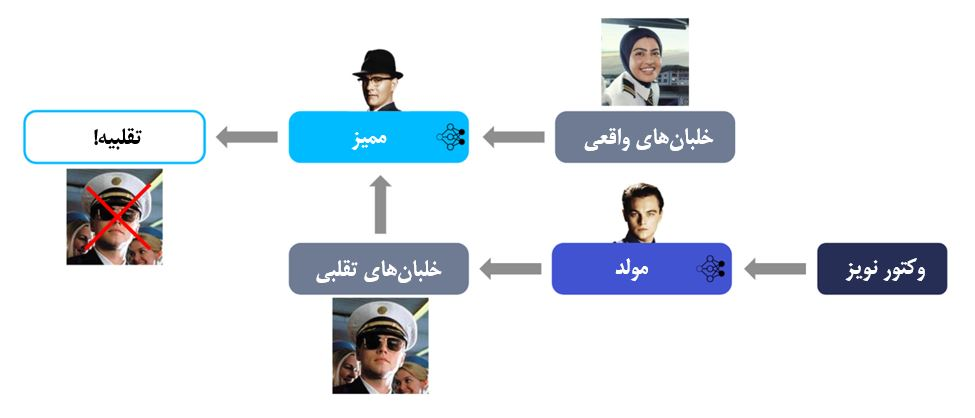
\includegraphics[width=1 \textwidth ]{images/gandiagram.jpeg}
	\caption{نحوه کارکرد شبکه مولد تخاصمی (گَن) به زبان «اگه می‌تونی منو بگیر»}
	\label{ganDiagram}
\end{figure}

\section{دیپ فیک \lr{Deepfake} چگونه ایجاد می شود؟}
از آنجاییکه \lr{Deepfake} با روش یادگیری ماشین کار میکند ، جهت جعل چهره ، \lr{Deepfake} به داشتن چند صد تصویر از حالات مختلف چهره هدف نیاز دارد. به منظور جابجایی چهره ؛ مجموعه داده های چهره هدف و ویدئو مقصد مورد نیاز است و این یکی از دلایلی است که اشخاص معروف و سیاستمداران بیشتر در خطر هستند و با سادگی با جستجویی سریع در اینترنت می توان تمام داده های مورد نیاز را بدست آورد.

بهترین روش حفاظت در برابر \lr{Deepfake} ، بستگی به خود شما دارد که آیا می خواهید عکس خود را از دید عموم حفظ کنید و یا آن را در اینترنت به صورت امن نگه دارید .

شاید تجمیع صدها تصویر از زوایای مختلف سبب ایجاد تصویری بسیار با کیفیت شود اما نبود این تعداد تصویر و زوایا نیز ، باز هم می تواند مورد استفاده  \lr{Deepfake} قرار گیرد با روش هایی همانند کشیدن تصاویر و فریم های چندگانه می توان شکاف ها را پر کرد. برنامه \lr{Everytime} آیفون تصویری که تهیه می کند ، حداقل 30 فریم در ثانیه ضبط می شود.

به هر حال برخی \lr{Deepfake} ها آنقدر هوشمند شده اند که کیفیت و کمیت مورد نظر تصاویر را می توانند بدست آوردند. به خصوص اگر زوایای صورت و چهره ها با ویدیو مقصد مورد نظر هماهنگ شود و اگر هم نباشد ممکن است ویدئو و تصاویر مقصد را با مبدا هماهنگ کنند.
	
\chapter{بد: جعل، تحقیر، و دروغ}\label{فصل دوم}
 	
 	پیشرفت فناوری دیپ‌فیک حالا به جاهای نگران‌کننده‌ای رسیده است. نه فقط عکس‌های تقلبی، که حالا می‌شود با این فناوری ویدیوهای فیک هم ساخت. خوشبختانه ویدیوهای دیپ‌فیک هنوز در ابتدای مسیرند و هرکس بخواهد آنها را بسازد، باید فریم به فریم ادیتشان کند. علاوه بر این، بیشتر می‌شود تغییرات ظاهری ایجاد کرد نه حرکات واقعی. اما با همه اینها، همین دو سال پیش کاربر ناشناسی در ردیت با نام مستعار \lr{\textcolor{blue}{deepfakes}}، چهره \textcolor{blue}{گَل گَدو}، بازیگر نقش واندر وومن را روی یک ویدیوی مستهجن گذاشت. کاربری دیگر در ردیت، اپی به نام \textcolor{blue}{فیک‌اپ } ساخت که با آن می‌شد به سادگی ویدیوهای فیک ساخت و به اشتراک گذاشت. امروز دیگر جایگزین کردن چهره یک نفر در ویدیو با یکی دیگر نه تنها کار سختی نیست، که نتیجه آن هم تا حد خیلی خوبی غیر قابل تشخیص است.
 	
 	در دنیایی که روزانه \textcolor{blue}{93 میلیون سلفی} در آن گرفته می‌شود، تصور کردن انواع سوءاستفاده‌ها و جرایمی که می‌شود با دیپ‌فیک انجام داد، خیلی کار سختی نیست: ساخت ویدیوهای مستهجن برای انتقام‌گیری، باج‌گیری، سرقت هویت، پخش اخبار دروغ. تازه، اینها تنها چند مثال از انبوه گزینه‌های ممکن است. در قالب تئوری، تک‌تک افرادی که عکس خودشان را در شبکه‌های اجتماعی به اشتراک بگذارند در آینده در مقابل چنین حملاتی آسیب‌پذیر خواهد بود. ویدیوهایی مثل \href{https://youtu.be/cQ54GDm1eL0}{سخنرانی فیک اوباما} را با این فناوری می‌شود در انواع و اقسام تولید کرد، افرادی که مستعد گول خوردن هستند را با آنها به راحتی گول زد، و بعد اعضای جامعه دو قطبی امروز حتی بیشتر از قبل با هم دشمن می‌شوند. وقتی اینترنت و شبکه‌های اجتماعی بی‌سانسور و کنترل نشده ما سرشار از دیپ‌فیک شوند، کل جامعه و زندگی‌های خصوصی تک‌تک ما در خطر خواهد بود.
 	

 	
\chapter{زشت: گرداب بی‌پایان رقابت‌ها}\label{فصل سوم}
\section{آیا ساخت دیپ فیک آسان است؟}
 	مثل هر نوع یادگیری ماشینی و غیر ماشینی دیگر، برای ساختن دیپ‌فیک‌های واقع‌گرایانه هم اول باید داده کافی جمع کرد. اما این خیلی هم کار ساده‌ای نیست. کوین روز (\lr{Kevin Roose})، یکی از نویسندگان ستون فناوری در نیویورک تایمز، تصمیم گرفت با دادن یک سری ویدیو از خودش به اپلیکیشن فیک‌اپ، خودش امتحان کند. دیپ‌فیکی که او با این روش از خودش ساخت بامزه بود، اما آنقدر واقعی نبود که آدم را گول بزند. بنابراین به نظر می‌رسد که فعلا، فقط از اشخاص مشهور می‌شود دیپ‌فیک   \textcolor{blue}{«واقعی» }ساخت؛ یعنی آنهایی که کلی ویدیوی باکیفیت ازشان در سطح وب وجود دارد. اما همین هم چیز کمی نیست؛ مثلا دیپ‌فیک‌ سیاستمداران می‌تواند بین صدها میلیون آدم دست به دست بچرخد و نتایج زیانباری برای وقایع سیاسی مهم داشته باشد؛ مثلا برای نتایج انتخابات ریاست جمهوری آمریکا در سال 2020.
\section{میتوان دیپ فیک ها را شکار کرد؟} 	
 	احتمال بروز چنین اتفاقاتی، بار سنگینی بر دوش فناوری‌های تشخیص و شکار دیپ‌فیک گذاشته است. متخصصان مختلف دارند همه تلاششان را می‌کنند تا ابزارهای قدرتمندی برای تشخیص دیپ‌فیک بسازند. مثلا پژوهشگران دانشگاه واشنگتن، سایت \textcolor{blue}{\href{http://www.whichfaceisreal.com/learn.html}{«کدام چهره واقعی است»} } را ساخته‌اند که در آن می‌توانید بعد از خواندن مطلبی در مورد نحوه تشخیص تصاویر دیپ‌فیک، سعی کنید بین یک سری عکس‌های واقعی و جعلی، واقعی‌ها را تشخیص دهید. کایل مک‌دانلد هم در یک پست وبلاگ در مورد همین مسئله توضیح داده است. گروهی از محققان یک دیتاست عظیم ویدیویی جمع کرده‌اند که قرار است در علوم قانونی (\lr{Forensics}) برای تشخیص جعل عکس، نقش محک و معیار را داشته باشد. استارتاپ دیپ‌تریس (\lr{\href{https://www.deeptracelabs.com}{Deeptrace}})، مبارزه با خطرات سایبری دیپ‌فیک را به عنوان هدف خود برگزیده و گزارشی در مورد وضعیت دیپ‌فیک در سال 2018 ارائه کرده است. \href{https://edition.cnn.com/2019/04/26/tech/ai-deepfake-detection-2020/index.html}{هنری فرید }در دارت‌ماوت دارد نرم‌افزاری برای شناسایی دیپ‌فیک‌های ویدیویی سیاسی می‌سازد. \href{https://www.usatoday.com/story/tech/2019/05/13/deepfakes-why-your-instagram-photos-video-could-be-vulnerable/3344536002/}{سیوی لیو }با همکاری آژانس پروژه‌های پژوهشی پیشرفته دفاعی (دارپا)، در حال توسعه نرم‌افزاری است که بتواند دیپ‌فیک‌های ویدیویی را شناسایی کرده و از انتشار و رواج آنها جلوگیری کند.
\section{نتیجه این شکار دیپ فیک ها  چیست؟} 
 	دیپ‌فیک‌ها درست مثل ویروس‌های کامپیوتری هستند. به محض اینکه یکی راه شناسایی‌ ویروسی را پیدا کند، فوری یک نفر دیگر می‌آید و راهی برای دور زدن راهکار نفر قبلی پیدا می‌کند. این قایم‌موشک‌بازی بین جعل‌کننده‌ها و تشخیص‌دهنده‌ها رقابتی است که تا ابد ادامه خواهد داشت. یک جورهایی، انگار خود این دو گروه با هم یک \lr{GAN} عظیم و بی‌پایان می‌سازند!
 	
\section{تهدید دیپ فیک \lr{Deepfake} چه قدر جدی است؟}
اما تهدید \lr{deepfakes}، واقعا تا چه حد پیچیده و جدی است؟ اگر در آینده اعتقاد به این پیدا کنیم که اکثر ویدئو ها جعلی هستند پس به چه چیز می توانیم اعتماد کنیم . تفاوت میان دروغ و درستی چگونه قابل تشخیص خواهد بود؟

هانی فرید می گوید: “مردم باید آگاه باشند که این چیزها وجود دارند اما باید درک کنند که ما با فناوری همراه هستیم، و اینکه چه چیزی می تواند و چه چیزی نمی تواند جعلی باشد.” ،  “مردم ممکن است یکباره خشمگین شوند و شروع به دیوانگی کنند. اما باید بتوانند این احساسات را کنترل کرده و سطح شناخت خود از اشخاص دور و برشان بالا ببرند به جای اینکه به ویدیوها و تصاویر جعلی اکتفا کنند .”\cite{asrIran}
 	
 	
 		\begin{figure}
 			\begin{center}
 					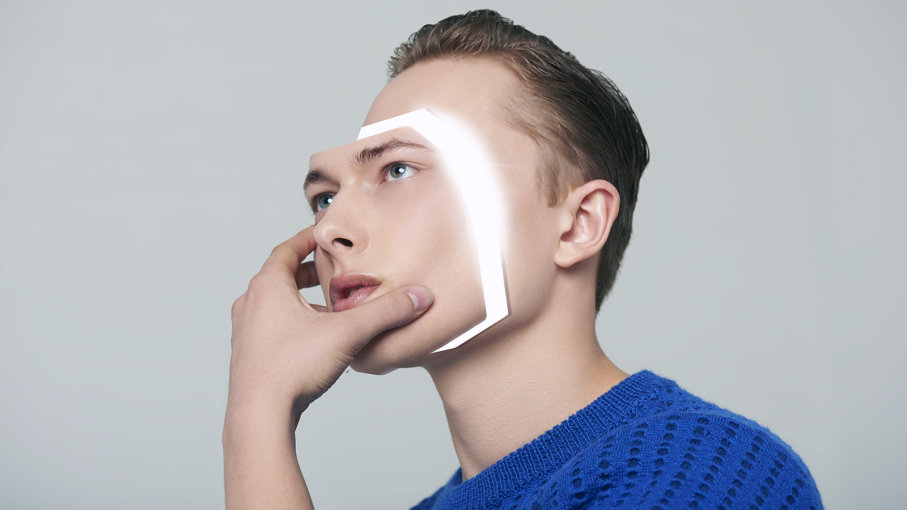
\includegraphics[width= 1 \textwidth]{images/tahdid.jpg}
 				\caption{تهدید دیپ‌فیک ها }
 				\label{tahdid}
 			\end{center}
 		\end{figure}
 
 	
\section{آیا \lr{Deepfakes} مهمترین تهدید در آینده خواهد بود؟}
بله واقعیت دارد \lr{Deepfakes} خطرناک است و ممکن است به نوعی تهدیدی جدی برای اشخاص مشهور ، سیاستمداران و یا حتی مردم عادی به شمار آید. ولی این فقط \lr{Deepfakes} نیست که باید از آن ترسید ، تهدیدهای بزرگتر دیگری هستند که اکثریت مردم عادی را نیز هدف قرار داده اند . همین دو سال اخیر بود که موضوع حفظ حریم شخصی توسط فیسبوک و گوگل به شدت زیر سوال رفت و به دنبال آن باگ امنیتی فیستایم اپل و برنامه هایی که بر روی موبایل ها خواسته و ناخواسته نصب می شوند و تمام اطلاعات و فعالیت های کاربران را با اهداف تجاری یا سوء استفاده های دیگر رصد میکنند. فن آوری ها به سرعت پیشرفت می کنند و به راحتی میان مردم منتشر می گردند؛ اما هنوز قوانین جامع و کاملی برای نحوه استفاده از آن ها وجود ندارد ، هنوز حتی قانونگذاران هم اطلاعات جامعی در خصوص دستگاه هایی که میان مردم عرضه می شود ندارند. پس \lr{deepfake} تنها دغدغه نخواهد بود .\cite{asrIran}
 	
\chapter{خوب: هوش مصنوعی شبه‌انسانی و تعاملات ارتباطی نو}\label{فصل چارم}
 	 جهان پر از دیپ‌فیک شاید مخوف و ناامن باشد؛ اما این تنها آینده ممکن نیست! دیپ‌فیک کاربردهای مثبتی هم دارد؛ دیپ‌فیک می‌تواند نحوه ارتباطات را دگرگون کند و شکل‌های کاملا جدیدی از آن به وجود بیاورد. به عنوان مثال، تصور کنید فناوری تولید صدا با فناوری دیپ‌فیک ترکیب شود! حتی همین حالا هم دستیار گوگل می‌تواند با استفاده از یک مدل مولد برای تولید گفتار به نام ویو‌نت (\lr{\textcolor{blue}{Wavenet}})، با لحن و صدای جان لجندصحبت کند. استارتاپ‌های لایربرد (\lr{\textcolor{blue}{Lyrebird}})و ماجولیت (\lr{\textcolor{blue}{Modulate}}) می‌توانند فقط با چند ساعت آموزش دیدن، یاد بگیرند مثل شما حرف بزنند! حتی فناوری بایدو (\lr{\textcolor{blue}{Baidu}}) می‌تواند تنها در 3.‌7 ثانیه صدای افراد را شبیه‌سازی کند. در آینده‌ای نه چندان دور، سخنگوهای هوشمندی خواهیم داشت که نه تنها می‌توانند با صدای خواننده‌های مورد علاقه‌مان صحبت کنند، که بلدند وقتی خودمان سر کار نیستیم، به جای ما جواب تلفن را بدهند!
 	
 حتی تولید ویدیوهای فیک هم الزاما چیز بدی نیست. شرکت سینتزیا (\lr{Synthesia}) ، ویدیوی دیپ‌فیکی از دیوید بکهام را برای یک کمپین حمایتی مالاریا تولید کرده است. استارتاپ دیتاگرید (\lr{DataGrid}) توانسته تصویر کل بدن آدم‌هایی که وجود خارجی ندارند را کامل بسازد، و پژوهشگران دانشگاه برکلی کالیفرنیا با کمک دیپ‌فیک توانسته‌اند حرکات مختلف رقص را روی بدن افراد مختلف اجرا کنند.


	 تصور کنید شخصیت‌های تاریخی‌ای که رویتان تاثیر گذاشته‌اند با شما حرف بزنند. تصور کنید عزیزانی که از دنیا رفته‌اند دوباره به پیشتان برگردند. و اگر هنوز دارید در آرزوی رفتن به دنیای هری‌پاتر می‌سوزید، تصور کنید همه آن پرتره‌های متحرک هاگوارتز واقعا وجود داشته باشند!
	
\chapter{جمع‌بندی}\label{فصل پنجم}
	 فرنک ابگنیل فیلم «اگه میتونی منو بگیر»، یک شخصیت واقعی است که وقتی سرانجام از زندان آزاد شد، چهار دهه از عمرش را به کار کردن در \lr{FBI} \LTRfootnote{Federal Bureau of Investigation}روی جعل‌، اختلاس، جرم‌های مالی، و جرم‌های امنیت سایبری گذراند. ابگنیل در \textcolor{blue}{\href{https://www.youtube.com/watch?v=vsMydMDi3rI}{سخنرانی‌ای در گوگل}} گفته که «فناوری، زاینده جرم است. همیشه همین بوده و همیشه هم چنین خواهد بود». با اینحال، او می‌گوید که این هکرها نیستند که امنیت اطلاعات شرکت‌ها را پایین می‌آورند؛ بلکه مقصر آن کارمندان سهل‌انگاری در آن شرکت هستند که کاری که قرار نبوده بکنند را کرده‌اند، یا اینکه نتوانسته‌اند کاری که قرار بوده بکنند را انجام دهند.
	 
	 	
	همین اتفاق برای دیپ‌فیک هم می‌افتد: مهم نیست دیپ‌فیک‌ها چقدر واقع‌گرایانه‌تر شوند یا دقت فناوری‌های ضد دیپ‌فیک تا چه حد افزایش پیدا کند؛ آسیب اصلی ناشی از این دیپ‌فیک‌ها کار انسان‌هایی هست که آنها را می‌سازند، ساخته‌های دروغین را باور می‌کنند، و چیزی که بدون تحقیق، درست فرض کرده‌اند را نشر می‌دهند. به جای اینکه انگشت اتهام را به سمت خود فناوری دیپ‌فیک بگیریم، باید ببینیم چطور می‌شود کاری کرد که افراد در مورد چیزهایی که در اینترنت می‌بینند با دید انتقادی‌تری قضاوت کنند و هنگام به اشتراک‌گذاری‌ در شبکه‌های اجتماعی هوشمندانه‌تر عمل نمایند. اثرات منفی دیپ‌فیک را نمی‌شود انکار کرد؛ اما باید چشم‌هایمان را به بخش‌های مثبت‌تر هوش مصنوعی بدوزیم و پتانسیلی که دیپ‌فیک برای ایجاد روش‌های ارتباطی جدید و بهتر کردن زندگی‌هایمان دارد را به مسیر درست هدایت کنیم.

\begin{thebibliography}{9}
	\latin
	\bibitem{queraMag}
	\lr{https://medium.com/twentybn/deepfake-the-good-the-bad-and-the-ugly-8b261ecf0f52}
	\bibitem{asrIran}
\lr{https://www.asriran.com/fa/news/673335/deepfake}
	.
	.
\end{thebibliography}
 	
\end{document}
